This section describes how actors can interact with Cracker in order to use all the features implemented in the app. The focus of this part is on the front-end and we show the operations that can be performed by the actors without taking care of the system architecture behind the app.

\vspace{6mm}

\subsection{Login}
\begin{figure}[h]
\centering
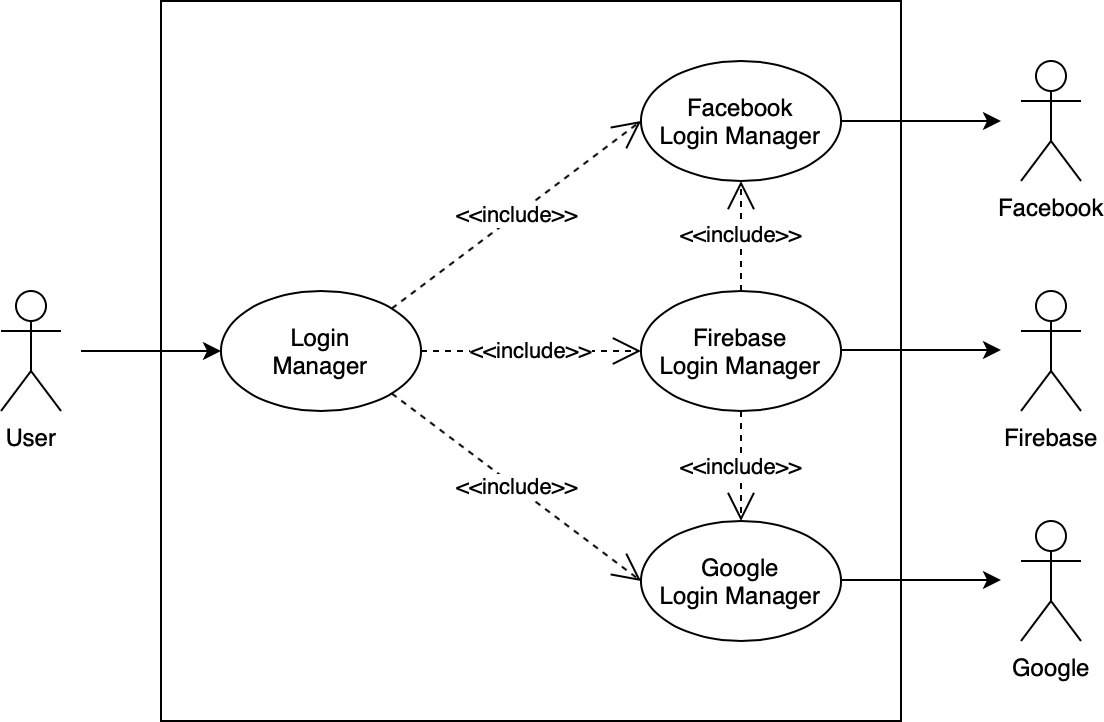
\includegraphics[width=\textwidth]{img/usecases/login}
\end{figure}

\clearpage

{\renewcommand{\arraystretch}{2}
{\begin{center}
\begin{tabular}{ | m{4cm} | m{9cm} | } 
 \hline
 {\centering{\textbf{Name}}} & Login \\
 \hline
 {\centering{\textbf{Actor}}} & User \\
 \hline
 {\centering{\textbf{Entry Condition}}} & Guest with login credentials \\
 \hline
 {\centering{\textbf{Goal}}} & 1 \\
 \hline
 {\centering{\textbf{Event flow}}} & \begin{itemize}[leftmargin=*]
 	\item The user opens the application
	\item The user presses ”Login with Facebook” (or "Login with Google") located in the welcome screen
	\item The user is redirected on Facebook (or Google) to enter credentials
	\item The app logs in through Facebook (or Google)
	\item The app login into Firebase using Facebook (or Google) account 
	\end{itemize} \\	
 \hline
 {\centering{\textbf{Exit condition}}} & Actor becomes Logged User \\
 \hline
 {\centering{\textbf{Exceptions}}} & The user is not connected to the network or he hasn’t a Facebook or Google account \\
 \hline
\end{tabular}
\end{center}}

\clearpage

\subsection{View Up Next}
\begin{figure}[h]
\centering
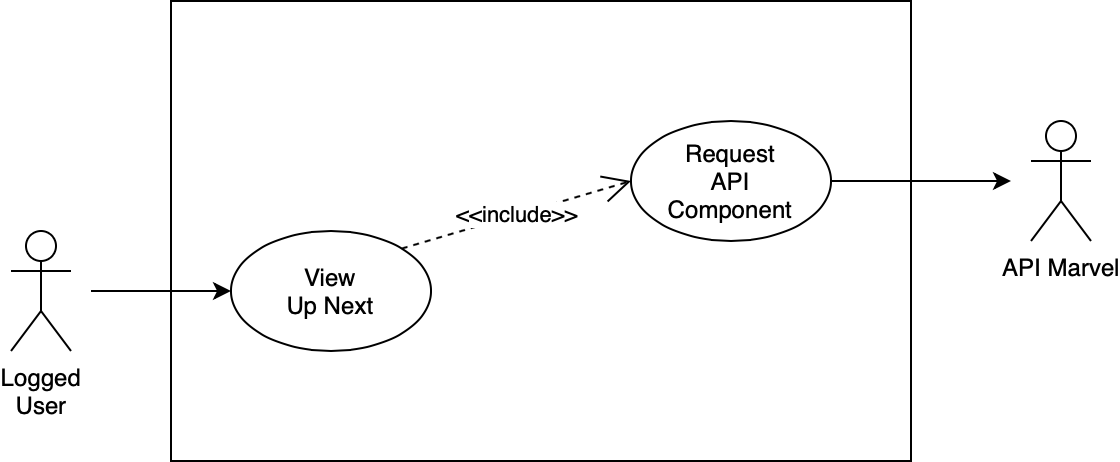
\includegraphics[width=\textwidth]{img/usecases/viewupnext}
\end{figure}

{\renewcommand{\arraystretch}{2}
{\begin{center}
\begin{tabular}{ | m{4cm} | m{9cm} | } 
 \hline
 {\centering{\textbf{Name}}} & View Up Next \\
 \hline
 {\centering{\textbf{Actor}}} & Logged User \\
 \hline
 {\centering{\textbf{Entry Condition}}} & The user logged in correctly \\
 \hline
 {\centering{\textbf{Goal}}} & 9 \\
 \hline
 {\centering{\textbf{Event flow}}} & \begin{itemize}[leftmargin=*]
 	\item The user opens the application
	\item The user presses on the "Up Next" tab located on the Tab Bar
	\item The app shows the upcoming issues divided by being published this week, next week, this month
	\end{itemize} \\	
 \hline
 {\centering{\textbf{Exit condition}}} & The user reads the titles of the upcoming issues \\
 \hline
 {\centering{\textbf{Exceptions}}} & The user is not connected to the network so he cannot send a request to read the titles of the upcoming issues \\
 \hline
\end{tabular}
\end{center}}

\clearpage

\subsection{View To Read}
\begin{figure}[h]
\centering
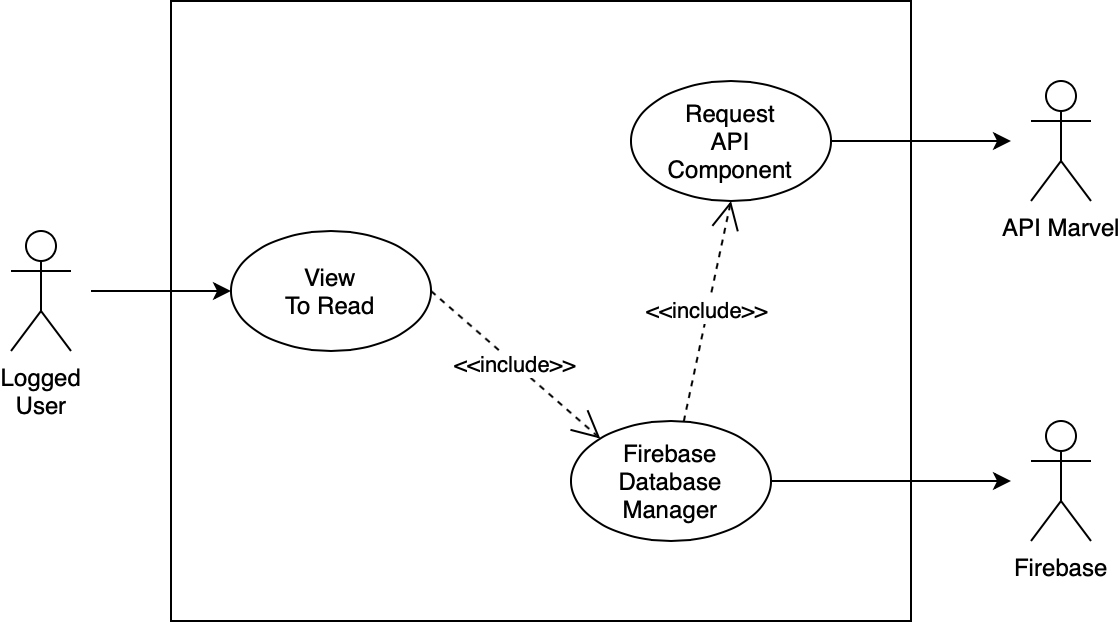
\includegraphics[width=\textwidth]{img/usecases/viewtoread}
\end{figure}

{\renewcommand{\arraystretch}{2}
{\begin{center}
\begin{tabular}{ | m{4cm} | m{9cm} | } 
 \hline
 {\centering{\textbf{Name}}} & View To Read \\
 \hline
 {\centering{\textbf{Actor}}} & Logged User \\
 \hline
 {\centering{\textbf{Entry Condition}}} & The user logged in correctly \\
 \hline
 {\centering{\textbf{Goal}}} & 6 \\
 \hline
 {\centering{\textbf{Event flow}}} & \begin{itemize}[leftmargin=*]
 	\item The user opens the application
	\item The user presses on the "To Read" tab located on the Tab Bar
	\item The app shows the next issue to read for all the series that the user is following
	\end{itemize} \\	
 \hline
 {\centering{\textbf{Exit condition}}} & The user sees the covers of the next issues he has to read \\
 \hline
 {\centering{\textbf{Exceptions}}} & The user is not connected to the network so he cannot send a request to get the next issues he has to read \\
 \hline
\end{tabular}
\end{center}}

\clearpage

\subsection{View Issue}
\begin{figure}[h]
\centering
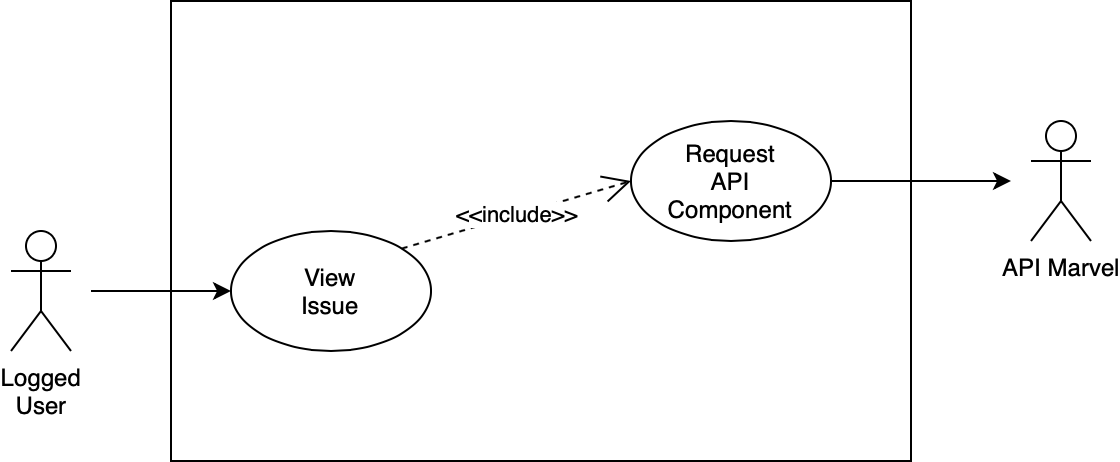
\includegraphics[width=\textwidth]{img/usecases/viewissue}
\end{figure}

{\renewcommand{\arraystretch}{2}
{\begin{center}
\begin{tabular}{ | m{4cm} | m{9cm} | } 
 \hline
 {\centering{\textbf{Name}}} & View Issue \\
 \hline
 {\centering{\textbf{Actor}}} & Logged User \\
 \hline
 {\centering{\textbf{Entry Condition}}} & The user logged in correctly \\
 \hline
 {\centering{\textbf{Goal}}} & 9 \\
 \hline
 {\centering{\textbf{Event flow}}} & \begin{itemize}[leftmargin=*]
 	\item The user opens the application and navigates through some screens
	\item The user presses on the button representing an issue in one of the screen where such a button is present
	\item The app shows the most important information about the issue
	\end{itemize} \\	
 \hline
 {\centering{\textbf{Exit condition}}} & The user reads the information about the issue \\
 \hline
 {\centering{\textbf{Exceptions}}} & The user is not connected to the network so he cannot send a request to get the information about the issue \\
 \hline
\end{tabular}
\end{center}}

\clearpage

\subsection{View Series}
\begin{figure}[h]
\centering
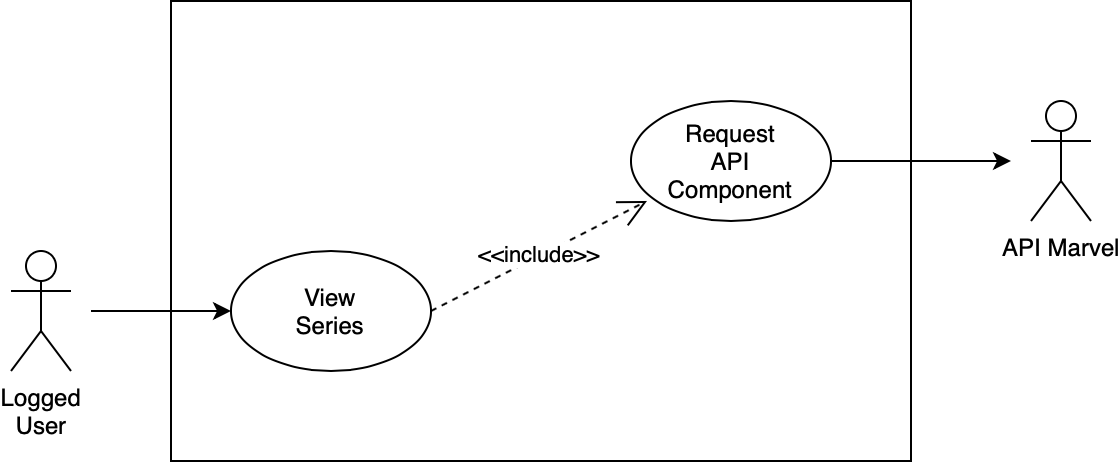
\includegraphics[width=\textwidth]{img/usecases/viewseries}
\end{figure}

{\renewcommand{\arraystretch}{2}
{\begin{center}
\begin{tabular}{ | m{4cm} | m{9cm} | } 
 \hline
 {\centering{\textbf{Name}}} & View Series \\
 \hline
 {\centering{\textbf{Actor}}} & Logged User \\
 \hline
 {\centering{\textbf{Entry Condition}}} & The user logged in correctly \\
 \hline
 {\centering{\textbf{Goal}}} & 9 \\
 \hline
 {\centering{\textbf{Event flow}}} & \begin{itemize}[leftmargin=*]
 	\item The user opens the application and navigates through some screens
	\item The user presses on the button representing a series in one of the screen where such a button is present
	\item The app shows the most important information about the series
	\end{itemize} \\	
 \hline
 {\centering{\textbf{Exit condition}}} & The user reads the information about the series \\
 \hline
 {\centering{\textbf{Exceptions}}} & The user is not connected to the network so he cannot send a request to get the information about the series \\
 \hline
\end{tabular}
\end{center}}

\clearpage

\subsection{Mark Issue as Read}
\begin{figure}[h]
\centering
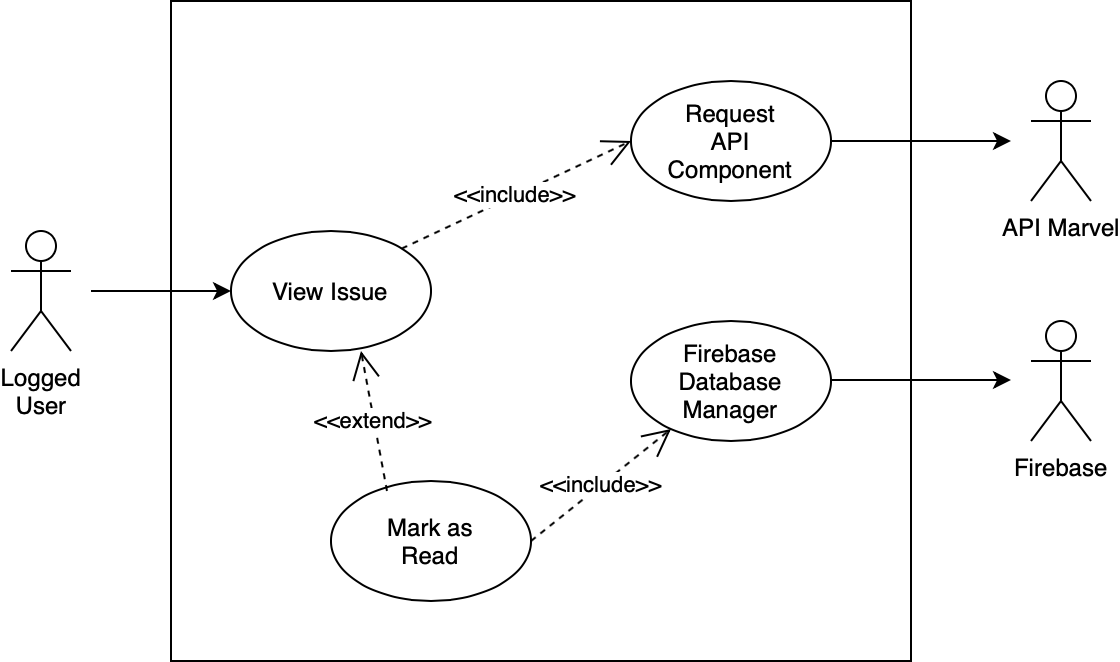
\includegraphics[width=\textwidth]{img/usecases/readissue}
\end{figure}

{\renewcommand{\arraystretch}{2}
{\begin{center}
\begin{tabular}{ | m{4cm} | m{9cm} | } 
 \hline
 {\centering{\textbf{Name}}} & Mark Issue as Read \\
 \hline
 {\centering{\textbf{Actor}}} & Logged User \\
 \hline
 {\centering{\textbf{Entry Condition}}} & The user logged in correctly \\
 \hline
 {\centering{\textbf{Goal}}} & 9 \\
 \hline
 {\centering{\textbf{Event flow}}} & \begin{itemize}[leftmargin=*]
 	\item The user opens the application and navigates through some screens, reaching one with information about an issue
	\item The user presses on the "Mark as read" button 
	\item The app records the action and updates the text of the button to "Mark as unread"
	\end{itemize} \\	
 \hline
 {\centering{\textbf{Exit condition}}} & The user marked an issue as read \\
 \hline
 {\centering{\textbf{Exceptions}}} & The user is not connected to the network so he cannot send a request to mark an issue as read \\
 \hline
\end{tabular}
\end{center}}

\clearpage

\subsection{Follow a Series}
\begin{figure}[h]
\centering
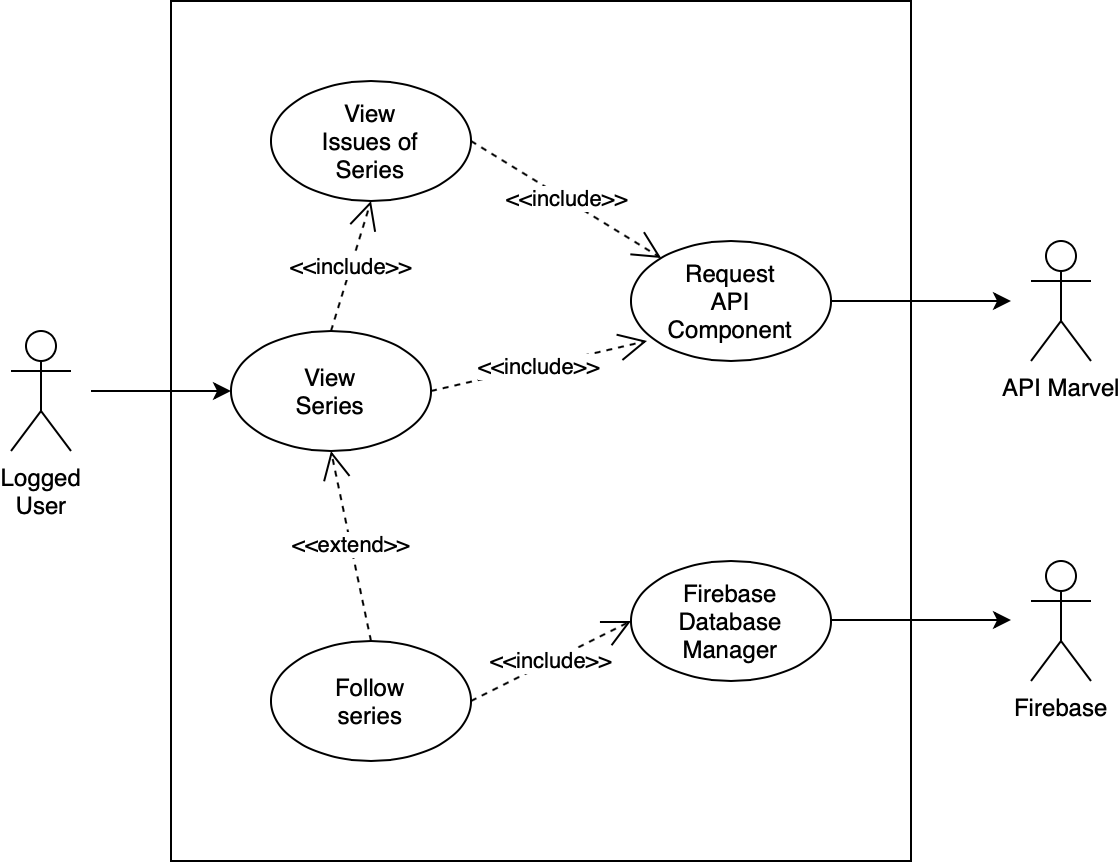
\includegraphics[width=\textwidth]{img/usecases/followseries}
\end{figure}

{\renewcommand{\arraystretch}{2}
{\begin{center}
\begin{tabular}{ | m{4cm} | m{9cm} | } 
 \hline
 {\centering{\textbf{Name}}} & Follow a Series \\
 \hline
 {\centering{\textbf{Actor}}} & Logged User \\
 \hline
 {\centering{\textbf{Entry Condition}}} & The user logged in correctly \\
 \hline
 {\centering{\textbf{Goal}}} & 9 \\
 \hline
 {\centering{\textbf{Event flow}}} & \begin{itemize}[leftmargin=*]
 	\item The user opens the application and navigates through some screens, reaching one with information about a series
	\item The user presses on the "Follow this series" button 
	\item The app records the action and updates the text of the button to "Unfollow this series"
	\end{itemize} \\	
 \hline
 {\centering{\textbf{Exit condition}}} & The user followed a series \\
 \hline
 {\centering{\textbf{Exceptions}}} & The user is not connected to the network so he cannot send a request to follow the series \\
 \hline
\end{tabular}
\end{center}}


\clearpage

\subsection{Search a Series}
\begin{figure}[h]
\centering
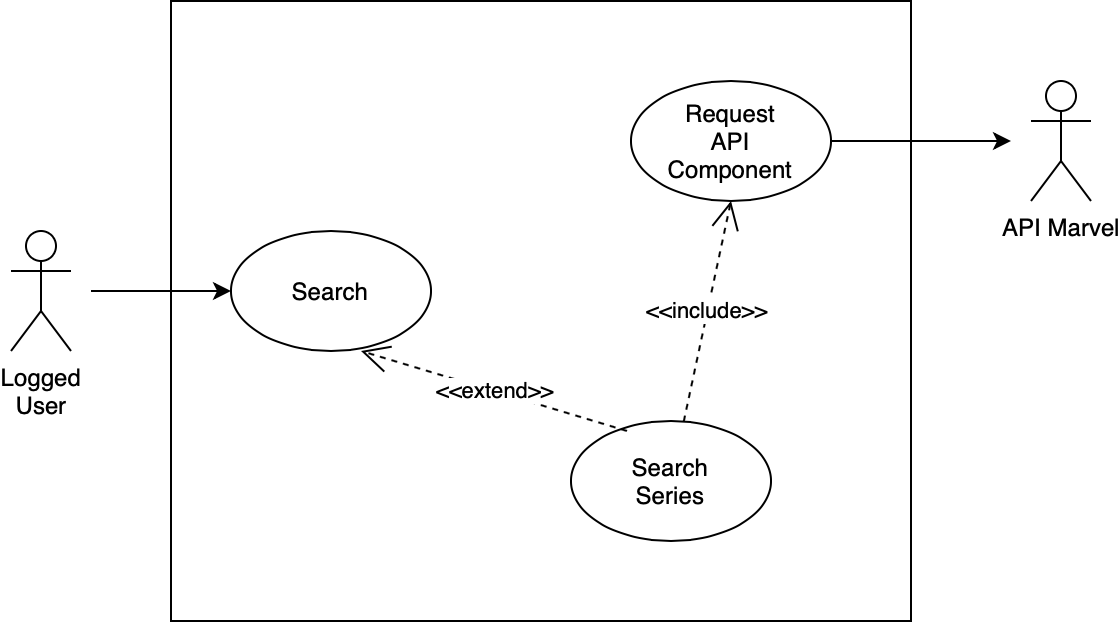
\includegraphics[width=\textwidth]{img/usecases/search}
\end{figure}

{\renewcommand{\arraystretch}{2}
{\begin{center}
\begin{tabular}{ | m{4cm} | m{9cm} | } 
 \hline
 {\centering{\textbf{Name}}} & Search a Series \\
 \hline
 {\centering{\textbf{Actor}}} & Logged User \\
 \hline
 {\centering{\textbf{Entry Condition}}} & The user logged in correctly \\
 \hline
 {\centering{\textbf{Goal}}} & 9 \\
 \hline
 {\centering{\textbf{Event flow}}} & \begin{itemize}[leftmargin=*]
 	\item The user opens the application
	\item The user presses on the "Search" tab located on the Tab Bar
	\item The app show a search bar
	\item The user presses on the search bar and types the name of a series
	\item The app shows the series whose name matches the one written by the user
	\end{itemize} \\	
 \hline
 {\centering{\textbf{Exit condition}}} & The user sees a list of series that match his input \\
 \hline
 {\centering{\textbf{Exceptions}}} & The user is not connected to the network so he cannot send a request to search for series \\
 \hline
\end{tabular}
\end{center}}

